\documentclass[tikz,border=8pt]{standalone}
% Shared look for every TikZ diagram. Load with % Shared look for every TikZ diagram. Load with % Shared look for every TikZ diagram. Load with \input{../../tools/tikz-style.tex}
\usepackage[T1]{fontenc}
\usepackage{lmodern}
\renewcommand{\sfdefault}{lmr}  % diagrams use the same serif as the text
\usetikzlibrary{arrows.meta, positioning, shapes.geometric, calc, fit, backgrounds}
\definecolor{cblue}{HTML}{4C78A8}
\definecolor{corange}{HTML}{F58518}
\definecolor{cgreen}{HTML}{54A24B}
\definecolor{cred}{HTML}{E45756}
\definecolor{cpurple}{HTML}{B279A2}
\definecolor{cgrey}{HTML}{6B6B6B}
\tikzset{
  every picture/.style={font=\sffamily, line width=1.2pt},
  box/.style={draw=#1, fill=#1!12, rounded corners=4pt, align=center, inner sep=7pt, minimum height=1.1cm},
  box/.default=cgrey,
  arrow/.style={-{Stealth[length=3mm]}, draw=cgrey, line width=1.4pt},
  title/.style={font=\sffamily\bfseries\Large},
  note/.style={font=\sffamily\small, text=cgrey, align=center},
}
\AtBeginDocument{\hyphenpenalty=10000 \exhyphenpenalty=10000}

\usepackage[T1]{fontenc}
\usepackage{lmodern}
\renewcommand{\sfdefault}{lmr}  % diagrams use the same serif as the text
\usetikzlibrary{arrows.meta, positioning, shapes.geometric, calc, fit, backgrounds}
\definecolor{cblue}{HTML}{4C78A8}
\definecolor{corange}{HTML}{F58518}
\definecolor{cgreen}{HTML}{54A24B}
\definecolor{cred}{HTML}{E45756}
\definecolor{cpurple}{HTML}{B279A2}
\definecolor{cgrey}{HTML}{6B6B6B}
\tikzset{
  every picture/.style={font=\sffamily, line width=1.2pt},
  box/.style={draw=#1, fill=#1!12, rounded corners=4pt, align=center, inner sep=7pt, minimum height=1.1cm},
  box/.default=cgrey,
  arrow/.style={-{Stealth[length=3mm]}, draw=cgrey, line width=1.4pt},
  title/.style={font=\sffamily\bfseries\Large},
  note/.style={font=\sffamily\small, text=cgrey, align=center},
}
\AtBeginDocument{\hyphenpenalty=10000 \exhyphenpenalty=10000}

\usepackage[T1]{fontenc}
\usepackage{lmodern}
\renewcommand{\sfdefault}{lmr}  % diagrams use the same serif as the text
\usetikzlibrary{arrows.meta, positioning, shapes.geometric, calc, fit, backgrounds}
\definecolor{cblue}{HTML}{4C78A8}
\definecolor{corange}{HTML}{F58518}
\definecolor{cgreen}{HTML}{54A24B}
\definecolor{cred}{HTML}{E45756}
\definecolor{cpurple}{HTML}{B279A2}
\definecolor{cgrey}{HTML}{6B6B6B}
\tikzset{
  every picture/.style={font=\sffamily, line width=1.2pt},
  box/.style={draw=#1, fill=#1!12, rounded corners=4pt, align=center, inner sep=7pt, minimum height=1.1cm},
  box/.default=cgrey,
  arrow/.style={-{Stealth[length=3mm]}, draw=cgrey, line width=1.4pt},
  title/.style={font=\sffamily\bfseries\Large},
  note/.style={font=\sffamily\small, text=cgrey, align=center},
}
\AtBeginDocument{\hyphenpenalty=10000 \exhyphenpenalty=10000}

\begin{document}
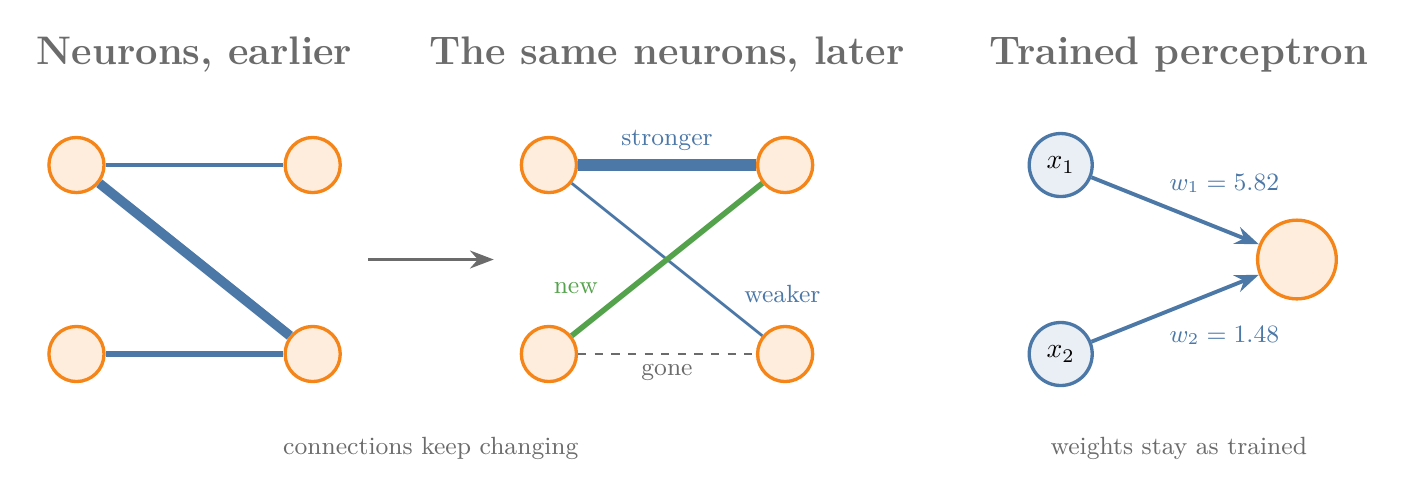
\begin{tikzpicture}
  \tikzset{cell/.style={circle, draw=corange, fill=corange!15, minimum size=0.7cm}}
  % neurons: earlier
  \node[title, cgrey] at (1.5,2.6) {Neurons, earlier};
  \node[cell] (a1) at (0,1.2) {}; \node[cell] (a2) at (0,-1.2) {};
  \node[cell] (a3) at (3,1.2) {}; \node[cell] (a4) at (3,-1.2) {};
  \draw[cblue, line width=1.2pt] (a1) -- (a3);
  \draw[cblue, line width=3.5pt] (a1) -- (a4);
  \draw[cblue, line width=2pt] (a2) -- (a4);
  % neurons: later
  \begin{scope}[xshift=6cm]
  \node[title, cgrey] at (1.5,2.6) {The same neurons, later};
  \node[cell] (b1) at (0,1.2) {}; \node[cell] (b2) at (0,-1.2) {};
  \node[cell] (b3) at (3,1.2) {}; \node[cell] (b4) at (3,-1.2) {};
  \draw[cblue, line width=4pt] (b1) -- node[above, note, cblue] {stronger} (b3);
  \draw[cblue, line width=1pt] (b1) -- node[pos=0.85, above right, note, cblue] {weaker} (b4);
  \draw[cgrey, dashed, line width=1pt] (b2) -- node[below, note, cgrey] {gone} (b4);
  \draw[cgreen, line width=2pt] (b2) -- node[pos=0.2, above left, note, cgreen] {new} (b3);
  \end{scope}
  \draw[arrow, cgrey] (3.7,0) -- (5.3,0);
  % perceptron
  \begin{scope}[xshift=12.5cm]
  \node[title, cgrey] at (1.5,2.6) {Trained perceptron};
  \tikzset{inp/.style={circle, draw=cblue, fill=cblue!12, minimum size=0.8cm}}
  \node[inp] (x1) at (0,1.2) {$x_1$}; \node[inp] (x2) at (0,-1.2) {$x_2$};
  \node[cell, minimum size=1cm] (s) at (3,0) {};
  \draw[arrow, cblue] (x1) -- node[above right, pos=0.4, font=\small] {$w_1 = 5.82$} (s);
  \draw[arrow, cblue] (x2) -- node[below right, pos=0.4, font=\small] {$w_2 = 1.48$} (s);
  \node[note, cgrey] at (1.5,-2.4) {weights stay as trained};
  \end{scope}
  \node[note, cgrey] at (4.5,-2.4) {connections keep changing};
\end{tikzpicture}
\end{document}
